\chapter{State of research}
\label{ch:state-of-research}
\textit{Operating system virtualisation} refers to all mechanisms that enable the creation of secure
and isolated application environments that run on top of a shared kernel. 
Conventionally, these mechanisms are baked into the kernel and are therefore part of the trusted computing base.
The kernel may expose these through its system-call interface, thereby allowing a user-space daemon 
program to provide an automated facility for creating and orchestrating sandboxed environments. 
This is the only feasible architecture on a general-purpose kernel such as Linux. 
Alternatively, the kernel may treat every software component, including its own subsystems, as an entity
to be wrapped in a sandbox. In that case, the concept of a process itself would have to 
satisfy all three virtualisation axioms. Examples of such operating systems include the seL4 \textit{microkernel}
- the first operating system to be formally verified as free of programming errors \cite{10.1145/1629575.1629596}, 
and Google's Fuchsia - described by \textcite{10.22667/JOWUA.2021.09.30.047}.

An application, referred to as a \textit{container},
is defined as an encapsulation of \enquote{[...] a software component and all its dependencies 
in a format that is self-describing and portable, so that any compliant container runtime can run it without extra 
dependencies, regardless of the underlying machine and the contents of the container} \cite[1]{oci-runtime-principles}.
A \textit{container runtime} is the user-space daemon program responsible for bringing this portable but 
static representation of an application into execution. In runtime, a container consists of a collection of processes 
that share a restricted view of the system's resources. For example, every container \enquote{believes}
it has a dedicated network stack with its own network interfaces, routing tables and packet-forwarding rules.
All processes in the container can access and manipulate that network stack, but no other process 
outside the container has that capability.
The container runtime configures this invariant and the operating system enforces it by 
namespacing system resources. The Open Containers Initiative (OCI) \cite{oci-website} has 
developed a runtime specification that standardises the operations a container runtime
needs to support. Most importantly, it must allow an external process called a \textit{container engine}
to hook into the lifecycle of a container. The container engine can use these hooks to manage 
all the containers on a single host system. In addition, the engine can attach network and storage 
to containers, thereby allowing processes in different sandboxes to share state and communicate 
with each other, if required. At the highest level of abstraction sits an orchestration platform that 
manages containers on multiple hosts by interacting with the container engine on each system.
This platform constantly monitors node and container health and dynamically multiplexes workloads 
based on various system properties of the cluster as to ensure maximum application availability.

It is important to note that, by definition, the kernel is assumed to be trustworthy. 
It has full control of all hardware resources and can access and modify the execution environment of every process on the system. 
In other words, noninterference between the kernel and user processes is not guaranteed.
Therefore, if the kernel is compromised, all processes on the system become untrustworthy.
It follows that if a process compromises the kernel, it transitively interferes with all other 
processes on the system. Hardening the operating system by implementing various security features such as
mandatory access control has been the primary approach for protection against such scenarios. 
However, the size of a monolithic general-purpose kernel is too large to adequately 
create a threat model that captures all possible vectors of attack. This problem is of particular concern 
to infrastructure providers whose entire business model revolves around consolidating hundreds of potentially 
malicious client applications on the same server, all of which share the same kernel and are allowed to directly interact with 
it via its system call interface. 

Unlike hardware virtualisation, this architecture does not use hardware emulation as an 
isolation primitive.
This means that shadow pages need not be maintained per virtual environment. Input-output operations need only 
traverse the kernel's stack without any address translations and with the additional 
performance benefit of direct memory access. As a result, the isolation overhead is lower 
compared to a virtual machine, which allows more applications to be consolidated onto a single server.
Furthermore, guests do not boot up complete operating system images, which reduces 
start times and memory consumption.
\textcite{10.1145/3126908.3126925} use containers in high-performance 
computing clusters to run user-defined compute jobs and show that the imposed performance penalties 
are, at most, negligible compared to vanilla processes that have no additional isolation.
\textcite{7095802} show the exact same thing and further conclude that the Docker container engine 
is resource-friendlier and faster than the Kernel Virtual Machine (KVM) when stressing the
\enquote{memory, IPC, network and filesystem subsystems} \textcite[1]{7095802} of the Linux kernel 
by running a database inside a virtual environment and evaulating its performance via the SysBench OLTP benchmark \cite{sysbench-oltp}.

Google's gVisor \cite{google-gvisor} attempts to sustain the performance advantages of 
containers whilst introducing an additional isolation boundary between the kernel and each container. The authors implement 
a substantial portion of the system call interface in a user-space process called Sentry.
Their dedicated container runtime calls out to Sentry instead of the kernel when issuing system calls.
\begin{figure}[H]
    \centering
    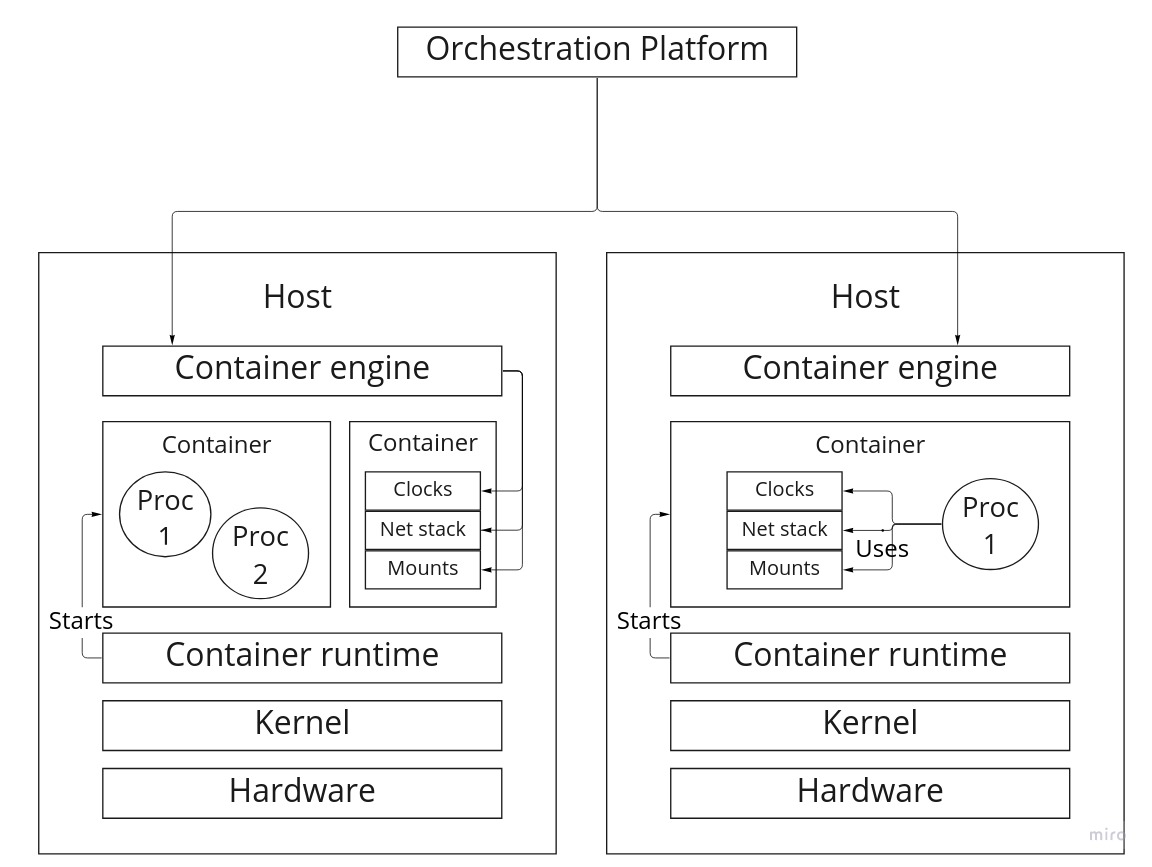
\includegraphics[width=0.55\textwidth]{images/fundamentals/cont-arch.jpg}
    \caption{Operating system virtualisation architecture using containers. The container runtime starts containers on a single host.
    A user process can see a bundle of resources allocated to it by the kernel. The kernel guarantees that a process 
    cannot see any other resources.
    The container engine manages all containers on a single system and allocates storage and networking to create explicit paths between containers.
    The orchestration platform talks to all engines inside a cluster to provide automatic workload management.}
    \label{images:fundamentals/cont-arch.jpg}
\end{figure}
However, \textcite{234857} show that network and memory allocation performance greatly suffer. 
This can be partially attributed to the fact that the Sentry process is implemented in a garbage-collected language 
and lacks the fine-grained optimisations contained in the Linux kernel.
\textcite{246288} take a different approach and try to fuse the security of virtual machines 
with the performance of containers by programming a custom virtual machine monitor 
called Firecracker that runs on top of KVM. Firecracker completely relies on the
Linux kernel for memory management, CPU scheduling and block I/O. To reduce its attack surface,
the virtual machine monitor sacrifices portability by supporting a limited set of emulated 
network and block devices. To further strengthen the noninterference boundary, the devices 
have configurable built-in rate limiters that can control the number of operations per second, e.g
disk/packets per second. Unlike a traditional container runtime, Firecracker's rate-limiting implementation
does not rely on the kernel, which makes its isolation boundary to the kernel stronger. 
\textcite{10.1145/3381052.3381315} evaluate both gVisor and Firecracker and show that 
the latter \enquote{[...] is effective at reducing the frequency of kernel code invocations, but had 
a much smaller impact on reducing the footprint of kernel code} \cite[12]{10.1145/3381052.3381315}. 

\textcite{10.1145/361011.361073} refer to the control program as a \textit{virtual machine monitor} that 
ensures isolation and noninterference by providing every program with an environment that is \enquote{[...] effect
identical with that demonstrated if the program had been run on the original machine directly} 
\cite[2]{10.1145/361011.361073}. This definition implies that a running program does not directly use
the bare metal resources available. Instead, resources are emulated by the virtual machine monitor at
the hardware level and presented as a dedicated physical system. Such an environment is called 
a \textit{virtual machine}.

\begin{figure}[H]
    \centering
    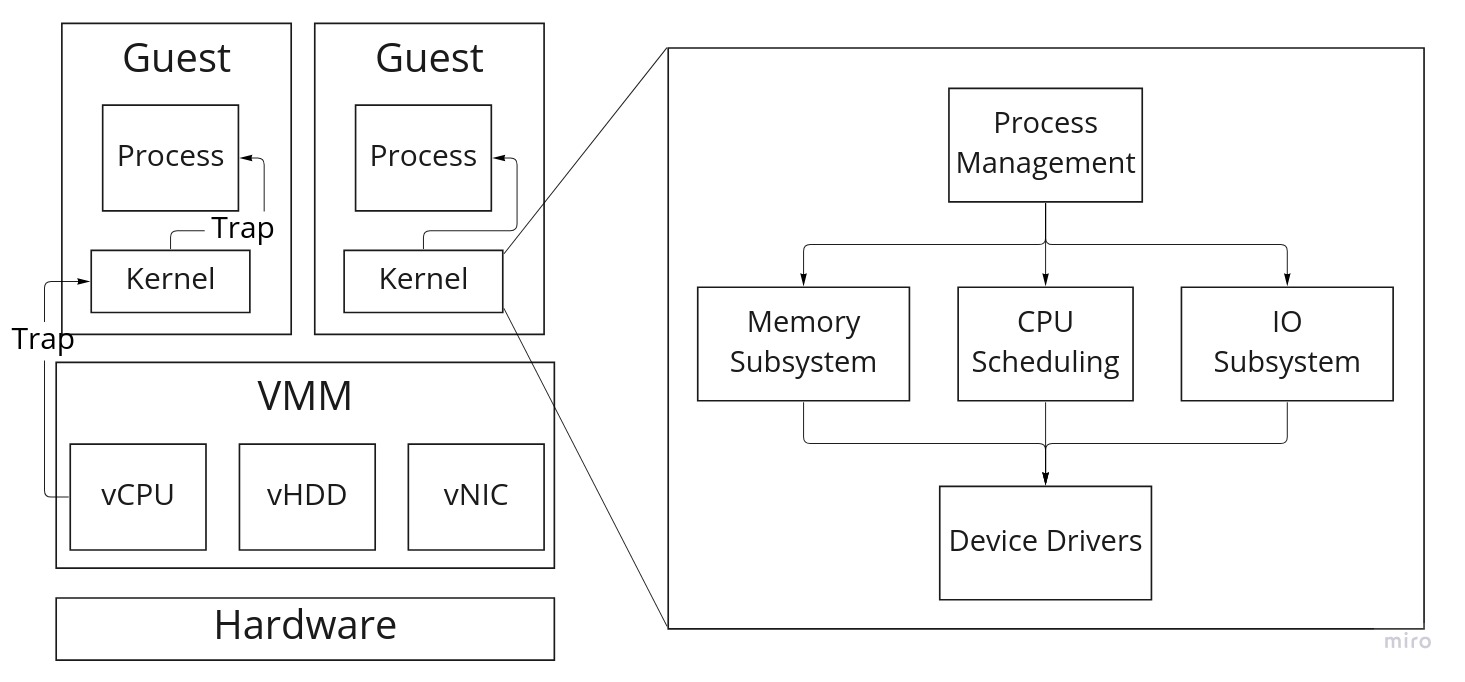
\includegraphics[width=0.70\textwidth]{images/fundamentals/full-virt-archh.jpg}
    \caption{Hardware virtualisation architecture. Each guest runs a complete operating system. 
             Privileged operations are trapped by the virtual machine monitor and emulated to provide hardware services.}
    \label{images:fundamentals/full-virt-archh.jpg}
\end{figure}

\textcite{10.1145/361011.361073} define a requirement that the instruction-set architecture of a computer
has to satisfy for it to be virtualisable. The instruction set must be segregated into three groups of
instructions - privileged, sensitive and innocuous. An instruction is privileged if it requires changing
the mode of execution from user to supervisor mode by means of a trap \cite{10.1145/361011.361073}. 
An instruction $i$ is control-sensitive if, when applied to the current processor state $S_1$, results
in a new state $i(S_{1}) = S_{2}$ such that the execution mode of $S_{2}$ does not equal that of $S_{1}$
or if $S_{2}$ has access to different resources than $S_1$ or both \cite{10.1145/361011.361073}. 
An instruction is behaviour-sensitive if its execution depends on the execution mode or its position
in memory \cite{10.1145/361011.361073}. An instruction is innocuous if it is not sensitive. 
Given these definitions, a computer is virtualisable \enquote{[...] if the set of sensitive instructions
for that computer is a subset of the set of privileged instructions} \cite[6]{10.1145/361011.361073}.
If this criterion is met, the virtual machine monitor can trap all sensitive instructions and emulate 
each via a homomorphism $i: C_{r} \rightarrow C_{v}$ that maps the state space of the processor without
the virtual machine monitor loaded $C_{r}$ to the state space with the virtual machine monitor loaded 
$C_{v}$ \cite{10.1145/361011.361073}. Innocuous instructions do not require protection, i.e a homomorphic
mapping, and are directly executed by the processor \cite{10.1145/361011.361073}.

Given the aforementioned homomorphism, a virtual machine can host a \textit{guest kernel} (Figure \ref{images:fundamentals/full-virt-archh.jpg}) that 
runs completely in user mode. 
Whenever the guest kernel attempts to execute a privileged instruction, 
the virtual machine monitor traps the attempt and emulates the instruction. 
Consequently, the guest kernel does not have to be a part of the trusted computing base. 
Even if it is compromised or encounters an unrecoverable error condition, other virtual machines 
remain unaffected. As a result, the isolation boundary between user programs running in different 
virtual machines is stronger compared to processes running on a shared kernel. 

In order to fully guarantee spatial noninterference between processes, the virtual machine monitor must 
be in full control of the host system's memory. There are two primary methods to do this - 
\textit{shadow paging} and \textit{extended page tables}. The former mechanism is considered first. 
The virtual machine monitor maintains a nested page table 
per guest, also called a \textit{shadow page table} \cite{10.5555/1204009}. 
In turn, the guest kernel maintains a page table per process. 
Whenever the guest kernel schedules a new process for execution, it modifies the \textit{page-table 
base register} to point to the page table for that process \cite{10.5555/1204009}. 
The virtual machine monitor intercepts this attempt and transparently updates the page table pointer to point to 
the guest's shadow page table corresponding to that process \cite{10.5555/1204009}. Note that 
the virtual machine monitor has to traverse the shadow page table for that guest in order to find the nested entry corresponding 
to the process. Afterwards, the memory management unit takes care of translating the virtual memory 
addresses of the guest and updating the \textit{translation lookaside buffer}.
Alternatively, the memory management unit may be \enquote{virtualisation-aware} in the sense that it knows 
there are two page tables it needs to traverse - the page table that maps guest virtual memory to guest 
\enquote{physical memory}, and the page table that maps guest physical memory to actual physical memory. 
The former is maintained by the guest kernel, whilst the latter is maintained by the virtual machine monitor.
The extended page table approach is up to 50\% faster than shadow paging \cite{2006PerformanceEO} because table
walks are done in hardware - by the memory management unit.
Nevertheless, maintaining page table data structures inside the virtual machine 
monitor and the guests leads to memory pressure, which is further amplified by the fact that 
guests, their applications and the virtual machine monitor all share the same physical memory \cite{10.5555/2490781}. 

The spatial noninterference property necessitates that the virtual machine monitor manage 
all input-output devices and their interactions with the guests. This is accomplished by the
already introduced trap-and-emulate pattern. When an application within a virtual machine 
issues a system call requesting some form of input-output, the request is processed by the 
I/O stack inside the guest. At the lowest level of the stack, the device driver issues a 
command to the device, typically by writing to memory specifically assigned to the device, or by
calling specific input-output instructions \cite{10.5555/2490781}. 
Either way, the virtual machine monitor intercepts this and traverses its own I/O stack, which 
remaps guest and real input-output addresses and forwards the request to a physical device \cite{10.1145/2063176.2063194}. 
After processing the request, the physical device triggers an interrupt that is caught by the virtual machine monitor and 
transformed into a virtual equivalent that is sent to the virtual machine that issued the request.
To reduce the overhead associated with interrupt processing, the virtual machine monitor can batch 
multiple events together and use a single interrupt to notify the guest kernel \cite{10.1145/2063176.2063194}.
Still, a request must traverse two input-output stacks. The same holds for the response.
In addition, hardware optimisations such as direct memory access are emulated in software, which 
further degrades performance. This, however, can be mitigated by integrating an input-output memory management 
unit that remaps all direct memory accesses of a device on the host to an address space in the guest.

The cost of hardware virtualisation becomes apparent when measuring same-host density
and boot times. \textcite{10.1145/3132747.3132763} consider memory consumption and on-disk image size
as the primary limiting factors. The authors measure the time it takes to create and boot
virtual machines using the Xen virtual machine monitor and show the negative effects that on-disk image size has 
by starting images with 
varying sizes by manually \enquote{[...] injecting binary objects into the uncompressed image file} \cite[3]{10.1145/3132747.3132763}. 
As the number of consolidated virtual instances increases and the image size grows, 
creation and boot times increase linearly.
Furthermore, the authors show that creating and starting a process directly on the host is, on average, 
two orders of magnitude faster. \textcite{10.1145/2151024.2151030} also evaluate Xen and state
that processing units spend 25\% of their total cycles in hypervisor mode instead of executing guest applications 
when running \enquote{[...] SPEC's first benchmark addressing performance evaluation of datacenter servers used in 
virtualised server consolidation} \cite[2]{10.1145/2151024.2151030}, which includes components 
such as a web, database and application server.
